% coding:utf-8

%FOSASTOC, a LaTeX-Code for a electrical summary of stochastic
%Copyright (C) 2013, Daniel Winz, Ervin Mazlagic

%This program is free software; you can redistribute it and/or
%modify it under the terms of the GNU General Public License
%as published by the Free Software Foundation; either version 2
%of the License, or (at your option) any later version.

%This program is distributed in the hope that it will be useful,
%but WITHOUT ANY WARRANTY; without even the implied warranty of
%MERCHANTABILITY or FITNESS FOR A PARTICULAR PURPOSE.  See the
%GNU General Public License for more details.
%----------------------------------------

\chapter{Kombinatorik}
\newpage

\section{Logik \& Mengenlehre}
Die Logik ist ein Teilgebiet der Mathematik und bedgründete das relativ
junge Teilgebiet der \gls{Mengenlehre} (engl. \emph{set theory}). 
Dass diese beiden Teilgebiete sich sehr ähnlich sind, zeigt sich 
unter anderem in ihren fast identischen Notationen.

Die Mengenlehre zeichnet sich insbesondere dadurch aus, 
dass es eine starke \gls{Abstraktion} zulässt.
Diese Eigenschaft ermöglicht es die Mengenlehre für viele Probleme
heranzuziehen. Die Stochastik ist nur eines von diesen.

\subsection{Begriffe der Mengenlehre}
\paragraph{Grundmenge und Grundraum}
In der Mengenlehre spricht man von der Grundmenge als die Menge aller
möglicher Elemente die in einer Menge erfasst werden können (von Neumann
Universum etc). Im Teilgebiet der Stochastik betrachtet man die
Elemente die in Mengen erfasst werden können als Eereignisse die eintreten
können. Die Gesamtheit all dieser möglichen Ereignisse nennt man 
\gls{Ereignisraum} oder Grundmenge, welche stets mit $\Omega$ 
notiert wird. 
Bei der Betrachtung eines Spiels mit einem Spielwürfel mit sechs Seiten 
wäre der Grundraum $\Omega=\{1,2,3,4,5,6\}$ und bei einem zweifachen
Münzwurf $\Omega=\{KK, KZ, ZK, ZZ\}$ usw.
\[  
	\Omega := \{x| P(x) \neq 0\}
\]

\paragraph{Teilmenge} 
Eine Menge $A$ heisst \gls{Teilmenge} von $B$, wenn jedes Element aus 
$A$ ein Element von $B$ ist. Somit kann eine solche Teilmenge $A$
auch die ganze Menge $B$ sein, d.h. $A=B$.
\[ 
	A \subseteq B
\]
\paragraph{Echte Teilmenge}
Eine \gls{echte Teilmenge} $A$ der Menge $B$ heisst echte Teilmenge, wenn
alle Elemente von $A$ in $B$ enthalten sind, aber die Menge $B$ noch
Elemente hat, die nicht in $A$ enthalten sind. In diesem Fall ist $B$ 
auch eine \emph{echte} Obermenge von $A$.
\[
	A \subset B
\]

\paragraph{Leere Menge} Eine \gls{leere Menge} ist eine Menge welche 
keinerlei Elemente enthält.
\[  
	A = \{\} = \emptyset
\]

\paragraph{Schnittmenge} Eine Menge von Elementen die allesamt in
allen Mengen vorkommen, wird \gls{Schnittmenge} dieser Mengen genannt.
\[ 
	A \cap B
\]

\paragraph{Vereinigungsmenge} Die Menge aller Elemente einer Menge
von Mengen wird als \gls{Vereinigungsmenge} bezeichnet.

\paragraph{Gleiche Menge} Wenn zwei Mengen die gleichen Elemente
enthalten und keine weiteren, so sind diese die \gls{gleiche Menge}.
\[  
	A = B 
	\quad \Leftrightarrow \quad 
	\forall x (x \in A \leftrightarrow x \in B)
\]

\paragraph{Differenzmenge}
Eine Menge die alle Elemente einer Menge enthält ohne jene die auch
in einer weiteren Menge vorkommen, wird als \gls{Differenzmenge} 
bezeichnet.
\[  
	A \setminus  B
\]

\newpage
\begin{figure}[h!]
	\centering
	\begin{subfigure}[b]{0.45\textwidth}
		\centering
		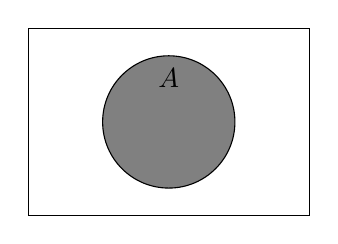
\begin{tikzpicture}[scale=0.7]
			\fill[white] (-2.55,-1.7) rectangle (2.55,1.7);
			\draw (-2.55,-1.7) rectangle (2.55,1.7);
			\fill[gray] (0,0) circle (1.2cm);
			\draw (0,0) circle (1.2cm);
			\draw (0,0.8) node {$A$};
		\end{tikzpicture}
		\caption{$A$}
	\end{subfigure}
	\begin{subfigure}[b]{0.45\textwidth}
		\centering
		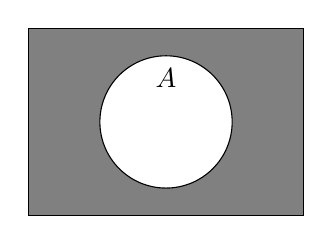
\begin{tikzpicture}[scale=0.7]
			\fill[gray] (-2.5,-1.7) rectangle (2.5,1.7);
			\draw (-2.5,-1.7) rectangle (2.5,1.7);
			\fill[white] (0,0) circle (1.2cm);
			\draw (0,0) circle (1.2cm);
			\draw (0,0.8) node {$A$};
		\end{tikzpicture}
		\caption{$A^C$}
	\end{subfigure}

	\rule[1mm]{0mm}{5mm}

	\begin{subfigure}[b]{0.45\textwidth}
		\centering
		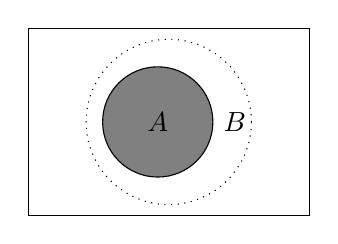
\begin{tikzpicture}[scale=0.7]
			\fill[white] (-2.55,-1.7) rectangle (2.55,1.7);
			\draw (-2.55,-1.7) rectangle (2.55,1.7);
			\draw[dotted] (0,0) circle (1.5cm);
			\fill[gray] (-0.2,0) circle (1cm);
			\draw (-0.2,0) circle (1cm);
			\draw (-0.2,0) node {$A$};
			\draw (1.2,0) node {$B$};
		\end{tikzpicture}
		\caption{$A \subseteq B$}
	\end{subfigure}
	\begin{subfigure}[b]{0.45\textwidth}
		\centering
		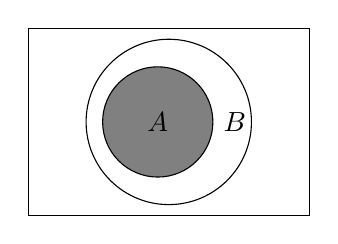
\begin{tikzpicture}[scale=0.7]
			\fill[white] (-2.55,-1.7) rectangle (2.55,1.7);
			\draw (-2.55,-1.7) rectangle (2.55,1.7);
			\draw (0,0) circle (1.5cm);
			\fill[gray] (-0.2,0) circle (1cm);
			\draw (-0.2,0) circle (1cm);
			\draw (-0.2,0) node {$A$};
			\draw (1.2,0) node {$B$};
		\end{tikzpicture}
		\caption{$A \subset B$}
	\end{subfigure}

	\rule[1mm]{0mm}{5mm}

	\begin{subfigure}[b]{0.45\textwidth}
		\centering
		\begin{venndiagram2sets}[tikzoptions={scale=0.7}]
    			\fillACapB
		\end{venndiagram2sets}
		\caption{$A \cap B$}
	\end{subfigure}
	\begin{subfigure}[b]{0.45\textwidth}
		\centering
		\begin{venndiagram2sets}[tikzoptions={scale=0.7}]
			\fillNotAorNotB
		\end{venndiagram2sets}
		\caption{${A\cap B}^C$}
	\end{subfigure}

	\rule[1mm]{0mm}{5mm}

	\begin{subfigure}[b]{0.45\textwidth}
		\centering
		\begin{venndiagram2sets}[tikzoptions={scale=0.7}]
			\fillA \fillB
		\end{venndiagram2sets}
		\caption{$A \cup B$}
	\end{subfigure}	
	\begin{subfigure}[b]{0.45\textwidth}
		\centering
		\begin{venndiagram2sets}[tikzoptions={scale=0.7}]
			\fillNotAorB
		\end{venndiagram2sets}
		\caption{$\overline{A \cup B}$}
	\end{subfigure}
	\caption{Die wichtigsten Definitionen der Mengenlehre graphisch
	erläutert mittels Venn-Diagrammen.}
\end{figure}

\section{Kombinatorik}
Im Teilgebiet der Stochastik gibt es einige Regeln die es in der 
Kombinatorik zu beachten gilt. Insbesondere sind dies die Axiome von
Kolmogorov.

\subsection{Axiome von Kolmogorov}
Der russische Mathematiker Andrei Nikolajevitsch Kolmogorov definierte
drei Axiome für die Wahrscheinlichkeitstheorie.
\begin{enumerate}
	\item \textbf{Nichtnegativität} \\
		Jedes Ereignis $A$ aus der Ergebnismenge $\Omega$ hat eine 
		reelle Eintrittswahrscheinlichkeit $P(A)$ von 
		$P(A) \geq 0$. Das bedeutet insbesondere, dass es 
		keine negativen Wahrscheinlichkeiten gibt.
		\[ P(A) \geq 0 \quad \text{für } A \in \Omega \] 
	\item \textbf{Normiertheit} \\
		Das sichere Ereignis der Ergebnismenge $\Omega$ hat eine
		Wahrscheinlichkeit von $P(\Omega)=1$. Dies sagt aus, dass
		sich immer etwas ereignen wird und dass das unmögliche
		Ereignis, die Wahrscheinlichkeit $P(\emptyset)=0$ hat.
		\[ P(\Omega) = 1 \]
	\item \textbf{Additivität} \\
		Die Wahrscheinlichkeit einer Vereinigung disjunkter 
		Ereignisse ist gleich der Summe der einzelnen 
		Wahrscheinlichkeiten. Dies kann als 
		$P(A_1 \dot\cup A_2  \dots ) = \sum P(A_i)$ 
		formuliert werden und wird als $\sigma$-Additivität
		bezeichnet.
		\[ P(A+B) = P(A)+P(B) \quad \text{falls } A \cap B = 0 \]
\end{enumerate}

\subsection{Stochastisch unabhängige Ereignisse}
\[ \begin{array}{c c l}
	P(A)	
		& \leq
		& 1 \\
	& & \\
	P(A) 
		& \geq 
		& 0 \\
	& & \\
	P(\Omega) 
		& = 
		& 1 \\
	& & \\
	P(A \cup B) 
		& = 
		& P(A) + P(B) \quad \text{Falls } A \cap B = 0 \\
	& & \\
	P(A \cup B) 
		& = 
		& P(A) + P(B) - P(A \cap B) \\
	& & \\
	P(A \cap B) 
		& = 
		& P(A) \cdot P(B) \\
	& & \\
	P(A \cap B \cap C) 
		& = 
		& P(A) \cdot P(B) \cdot P(C) \\
	& & \\
	P(A^C) 
		& = 
		& 1 - P(A)
\end{array} \]
	
\subsection{Diskrete Wahrscheinlichkeit}
\[ 
	P(E)
	= \frac{\text{Anzahl positiver Elementarereignisse für } E}{
		\text{Anzahl aller möglicher Elementarereignisse}}
\]

\section{Bedingte Wahrscheinlichkeit}
Bei bedingten Wahrscheinlichkeiten kann das Beyes'sche Theorem angewandt
werden. Mit Hilfe dieses Theorems kann die Wahrscheinlichkeit, dass $A$
einritt wenn $B$ eingetreten ist umgekehrt werden zur Formulierung dass
$B$ eintritt, gegeben es sei $A$ eingetreten.

\subsection{Beyes'sche Theorem}
\[ \begin{array}{c c l}
	P_B(A) 
		& = 
		& P(A|B) \\
	& & \\
	P(A|B)
		& = 
		& \displaystyle \frac{P(A \cap B)}{P(B)} 
			= \displaystyle 
			\frac{P(B|A) \cdot P(A)}{P(B)} \\
	& & \\
	P(B) 
		& = 
		& P(B|A) \cdot P(A) + P(B|A^C) \cdot P(A^C) \\
	& & \\
	P(B) 	
		& = 
		& P(B \cap A) \cdot P(A) + P(B|A^C) \cdot P(A^C)
\end{array} \]

\newpage
\subsection{Tabelle zu bedingten Wahrscheinlichkeit}
Mit dem Beyes'schen Theorem kann eine tabellarische Übersich von
zwei bedingten Ereignissen erstellt werden, welche wiederum mittels
der Kolmogorv'schen Axiome bestimmt werden.

\begin{figure}[h!]
	\centering
	\begin{subfigure}[b]{0.75\textwidth}
		\centering
		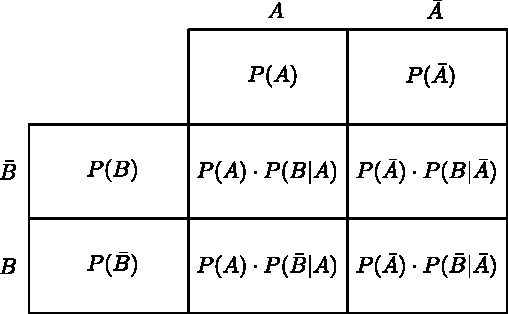
\includegraphics[width=1\textwidth]{bedingte-wahrscheinlichkeit.pdf}
	\end{subfigure}

	\rule[1mm]{0mm}{5mm}

	\begin{subfigure}[b]{0.75\textwidth}
		\centering
		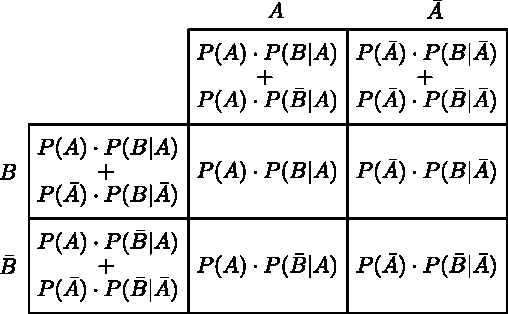
\includegraphics[width=1\textwidth]{bedingte-wahrscheinlichkeit-detail.pdf}
	\end{subfigure}
	\caption{Tabelle bedingter Wahrscheinlichkeiten.}
\end{figure}

\newpage
\begin{figure}[h!]
	\centering
	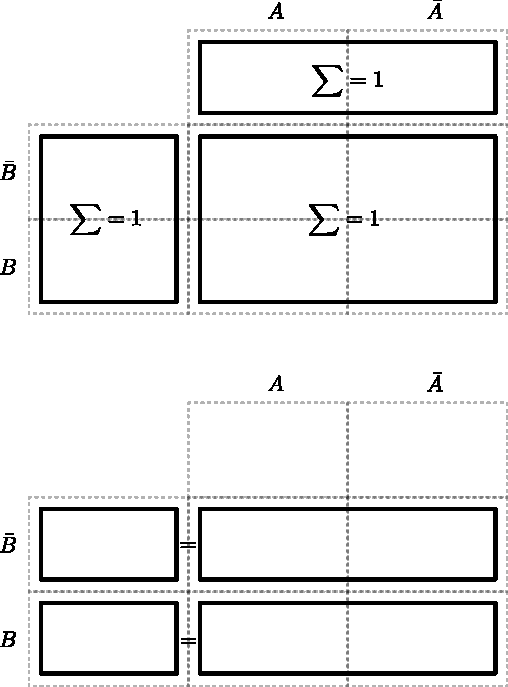
\includegraphics[width=0.65\textwidth]{bedingte-wahrscheinlichkeit-tipps.pdf}
	\caption{Hinweise zur Tabelle bedingter Wahrscheinlichkeiten.}
\end{figure}
